\documentclass[a4paper,11pt]{article}

\usepackage[utf8]{inputenc}    % Pour que LaTeX comprenne les accents.
\usepackage{times}             % Police de caractères
\usepackage[english]{babel}     % Traitement du texte adapté aux règles typographiques
                               % de la langue donnée en option (e.g., pour l'espacement
                               % après les ponctuations
\usepackage[T1]{fontenc}
\usepackage{amsmath, amsthm, amssymb} 
\usepackage{dsfont}  % pour les indicatrices 
\usepackage{graphicx} 
\usepackage{textcomp}  
\usepackage{enumerate}                             
\sloppy              % Ne pas faire déborder les lignes dans la marge


\newtheorem{lemma}{Lemma}
\newtheorem{cons}{Corollary}
\newtheorem{theo}{Theorem}

\theoremstyle{definition}
\newtheorem{definition}{Definition}
\newtheorem{process}{Process}

\theoremstyle{remark}
\newtheorem{remark}{Remark}

\newcommand{\R}{\mathbb{R}}
\newcommand{\M}{\mathcal{M}}
\newcommand{\N}{\mathcal{N}}
\newcommand{\C}{\mathcal{C}}
\renewcommand{\Pr}{\mathbb{P}}
\newcommand{\Esp}{\mathbb{E}}
\renewcommand{\P}{\mathbf{P}}
\newcommand{\pper}{p^{\mathrm{per}}}
\newcommand{\ptable}{p^{\mathrm{table}}}
\newcommand{\Cp}{\mathcal{C}^{\mathrm{per}}}
\newcommand{\Ca}{\mathcal{C}}

\title{Throwing needles on a coloured plane.}
\author{Thomas Bourgeat \and Marc Heinrich \and Paul Melotti 
\and Jean-Marc Robert}

\begin{document}
\maketitle

\begin{abstract} Colouring a table with $k$ colours, and throwing a needle
randomly on it gives a certain probablity that the endpoints fall on 
different colours. How can one make this probability maximal?
This problem is related to finite graphs having unit-lengthed edges, and 
some bounds on the optimal probability are deduced.\end{abstract}

\section{Introduction}

A well-known problem of geometric graph theory is the following: how many colors
are needed to color the plane so that no two points at unit distance are the 
same color? This is known as the Hadwiger-Nelson problem, and the answer to that
question is often refered as the \textit{chromatic number of the plane}. It 
seems that the problem was first stated by Nelson in 1950, and first published by 
Gardner in \cite{gardner}.
For a nice review about this problem and close relatives, see Soifer's book
\cite{soifer}. This question is still very mysterious to that day, and all that 
is known for sure is that the chromatic number of the plane is at least 4 and at
most 7.

The questions presented here may be seen as a probabilistic version of this 
problem, since we don't try to make \textit{every} unit-lengthed segment 
bichromatic but a large fraction of them.

We first state some definitions to clarify what kinds of colourings we will consider.
We will be interested in \textit{periodic} and \textit{asymptotic} colourings,
the latter being a generalization of the former.
\begin{definition}
\
\begin{enumerate}[i)] 
\item A $k$-\textit{colouring} of the plane is a measurable function $c$ from the euclidian 
plane~$\R ^2$ to the finite set $\{1, \dots , k \}$.

A \textit{colouring} is a $k$-colouring for some $k$.
\item The set of \textit{monochromatic needles} of a colouring $c$ is the set
\[ \M (c) = \{x,y \in \R ^2 \times \R ^2 \mid c(x) = c(y) \} \]
which is a measurable subset of $\R ^4$.
\end{enumerate}
\end{definition}

\begin{definition}
\
\begin{enumerate}[i)] 
\item A colouring $c$ is said to be \textit{periodic} if there are two free
vectors $(u,v)$ so that for any $x$ in $\R ^2$, $c(x+u)=c(x+v)=c(x)$. In that
case we note $\P_c$ the parallelogram formed on $u$ and $v$.
\item For a periodic coloring $c$, consider the following random variables:
let $A$ be a point chosen uniformly in $\P_c$, and $B=A + e^{i \theta}$ where
$\theta$ is a random angle taken uniformly in $[0;2 \pi[$ indepedently of $A$.

Then we note $\pper(c)$ the probability
$$\pper(c) = \Pr(c(A)=c(B)).$$
\end{enumerate}
\end{definition}

\begin{definition}
\
\begin{enumerate}[i)]\label{defas}
\item If $A$ is a measurable subset of $\R^2$ and $c$ a colouring, let $\N_A$ be
the set of \textit{needles inside} $A$, and $\M_A$ the set of \textit{monochromatic
needles inside} A:
\[\N_A = \{(x,y) \in A ^2 \mid d(x,y)=1\}, \]
\[\M_A (c) = \M (c) \cap \N_A. \]

\item  \label{asympt}The colouring $c$ is said to be \textit{asymptotic} if the ratio
$\frac{\lambda (\M_{[-R;R]^2})}{\lambda (\N_{[-R;R]^2})}$ 
converges to a limit $p(c) \in [0,1]$ as $R$ tends to infinity (where $\lambda$ 
is the Lebesgue measure on $\mathbb{R}^4$).
\end{enumerate}
\end{definition}

It should be clear that a periodic colouring $c$ is also an asymptotic colouring,
and $\pper(c)=p(c)$ in that case. However, contrary to $\pper(c)$, $p(c)$ is not
in general a probability and shouldn't be seen as such; we may call it an 
asymptotic probability.

Our aim will be to make $p(c)$ as small as possible, since it is not hard
to make it big.
\\

Some other defintions are needed in order to relate this problem to finite
graphs. In particular, we need to describe how a finite
graph can be ``well $k$-coloured'' even when its chromatic number is greater
than $k$.
\begin{definition}
\ 
\begin{enumerate}[i)]
\item For a finite graph $G=(V,E)$ and a $k$-colouring $c$ of the vertices of $G$, 
let $M_G(c)$ be the number of monochromatic edges in $G$ when couloured with $c$:
$$M_G(c) = \sum_{i \sim j} \mathds{1}_{c(i)=c(j)}.$$
where the sum is on the edges of $G$.

Then we define $m_k(G)$ as:
\[m_k(G) = \min_{c \ k-\mathrm{colouring \ of} \ G} \frac{M_G(c)}{|E|}.\]
\item A finite graph is said to be a \emph{unit distance graph} if it has 
an embedding in $\R^2$ in which all edges have length $1$.
\end{enumerate}
\end{definition}
In section~\ref{equiv} we prove the following:
\begin{theo} \label{ineg}
Let $\mathcal{G}$ be the set of unit distance graphs and $\Cp_k$ the set 
of periodic $k$-colourings of the plane, then
$$ \sup_{g \in \mathcal{G}} \ m_k(g) \leq \inf_{c \in \Cp_k} \ \pper(c) \leq \frac{1}{k}. $$
\end{theo}
The rest of the paper aims at proving the analogous theorem for asymptotic 
colourings, whose proof is ended in section~\ref{ext}:
\begin{theo} \label{ineg2}
Let $\mathcal{G}$ be the set of unit distance graphs and $\C_k$ the set 
of asymptotic $k$-colourings of the plane, then
$$ \sup_{g \in \mathcal{G}} \ m_k(g) \leq \inf_{c \in \C_k} \ p(c) \leq \frac{1}{k}. $$
\end{theo}

In section~\ref{appli} we study the particular cases $k=2,3$ are discussed,
and prove the following consiquence of the theorems:
\begin{cons}\label{con}
If \ $\inf_{c \in \Ca_k} \ p(c) = 0$ \ then the chromatic number of the
plane is at most $k$.
\end{cons}
We study in section~\ref{ext} the case of a finite table instead of the whole plane,
complete the proof of theorem~\ref{ineg2}, and give some remarks on possible 
generalizations to higher dimentions.

\section{Process equivalence}
\label{equiv}

Let $c$ be a periodic colouring, and consider the needle-throwing ``processes'':
\begin{process} \label{premier}
Consider the following random variables:
\begin{itemize}
  \item let $A$ be a point chosen uniformly 
  in $\P_c$ ;
  \item let $\theta$ be an independent angle chosen uniformly in $[0;2 \pi[$ ;
  \item let $B$ be $A + e^{i \theta}$.
\end{itemize}
\end{process}

Note that $B$ may fall outside of $\P_c$. In that case, $c(B)$ is 
defined using the periodicity of the colouring.
Our goal is to evaluate and minimize the probability that both ends have the 
same color.

We consider the following, second process that will be very useful in our 
proofs. The idea is to throw a unit distance graph on the 
plane, and then to choose a needle on that graph~:
\begin{process}
Given a unit distance graph $G = (V,E)$, embedded in the plane in 
a unit distance way. Label its edges with numbers from 
$1$ to $m$. The complex coordinates of the vertices of the $j^{th}$ edges are 
named $z_j $ and $z_j + e^{i.\theta_j}$. Choose~: 
\begin{itemize}
\item one point $A_0$ uniformly in $\P_c$ ;
\item an independent angle $\theta$ uniformly in $[0;2\pi[$ (to rotate the graph) ;
\item an independent integer $J$ in $[| 1;m|]$.
\end{itemize}
Then, rotate the graph by the angle $\theta$, translate it so that the origin 
falls on $A_0$, and take the needle $(A',B')$ corresponding to the $J^{th}$ 
edge of the obtained graph. In other words:
$$A' = e^{i.\theta} z_J + A_0, \ B' = e^{i.\theta} (z_J + e^{i.\theta_J}) + A_0.$$
\end{process}

\begin{lemma}\label{huitre}
Let $c_1$ and $c_2$ denote 
two colors. Then, we 
have~:\\
 $$\mathbb{P}(c(A) = c_1, c(B) = c_2) = \mathbb{P}(c(A') = c_1, c(B') = c_2) $$ \\
 In particular, the probability doesn't depend on the graph 
 chosen.
\end{lemma}

\begin{proof}
We call $\mathcal{A}(\P_c)$ the area of $\P_c$.

We prove the lemma by the following series of equalities:
\begin{eqnarray*}
& & \mathbb{P}(c(A') = c_1, c(B') = c_2) \\
  &=& \frac{1}{m}\sum_{j=1}^{m} \mathbb{P}(c(A') = c_1, c(B') = c_2 | J=j)  \\
  &=& \frac{1}{m}\sum_{j=1}^{m}  \frac{1}{2\pi}\int_{\theta =0} ^{2\pi} \frac{1}{\mathcal{A}(\P_c)}\int_{A_0 \in \P_c} \mathbb{P}(c(A') = c_1, c(B') = c_2 | J=j, \theta, A_0) d\theta dx dy \\  
  &=& \frac{1}{m 2\pi \mathcal{A}(\P_c)}\sum_{j=1}^{m}\int_{\theta =0} ^{2\pi} \int_{A_0 \in \P_c} \mathds{1}(c(A_0 + z_i e^{i\theta}) = c_1, c(A_0 +z_j e^{i\theta} + e^{i (\theta + \theta_j)}) = c_2) d\theta dx dy \\  
    &=& \frac{1}{m 2\pi \mathcal{A}(\P_c)}\sum_{j=1}^{m} \int_{\theta =0} ^{2\pi} \int_{A_0 \in \P_c} \mathds{1}(c(A_0) = c_1, c(A_0 + e^{i (\theta + \theta_j)}) = c_2 ) d\theta dx dy \hspace{1 cm} (*)\\ 
    &=& \frac{1}{m 2\pi \mathcal{A}(\P_c)}\sum_{j=1}^{m} \int_{\theta =0} ^{2\pi} \int_{A_0 \in \P_c} \mathds{1}(c(A_0) = c_1, c(A_0 + e^{i \theta}) = c_2 ) d\theta dx dy \\ 
    &=& \frac{1}{2\pi \mathcal{A}(\P_c)}\int_{\theta =0} ^{2\pi} \int_{A_0 \in \P_c} \mathds{1}(c(A_0) = c_1, c(A_0 + e^{i \theta}) = c_2 ) d\theta dx dy \\ 
\end{eqnarray*}
Which gives exactly the same probability as the first process.

Equality $(*)$ is justified by the periodicity of our colouring.
\end{proof}

\begin{proof}[Proof of theorem~\ref{ineg}]
Consider a graph $g$ coloured with $k$ colours. When one chooses a needle
randomly on this graph the probability that both ends have the same
colours is clearly greater than $m_k(g)$. Applying lemma \ref{huitre} with $g$, 
it follows from the description of the second process that the probability 
$\pper(c)$ for any colouring $c$ is greater than $m_k(g)$.

Now to get the right-hand side of the theorem, let $\P$ be a square of side $R$,
and cut $\P$ into $n^2$ squares of side $R/n$. Let $C$ be a \textit{random} 
colouring obtained by assigning to these $n^2$ smaller squares i.i.d. colours
taken uniformly in $\{1,\dots,k\}$ and repeating $\P$ to get a periodic 
colouring. Then one easily checks that for $R$ large enough and $R/n$ small
enough, for any needle $(A,B)$, $A$ and $B$ are in distinct small squares so
$$\Pr(C(A)=C(B)) = \frac1k$$
and an application of Fubini's theorem shows that
$$\Esp[\pper(C)] = \frac1k$$
so that there is a realisation $c_0$ with $\pper(c_0) \leq \frac1k$.
\end{proof}
We still don't know wether or not the left-hand inequality of theorem~\ref{ineg} is actually an equality. It is for 
$n=2$, as will be shown thereafter.

\section{Applications} \label{appli}
\subsection{2 colours} \label{2col}

With two colors, we consider an equilateral triangle as a unit distance graph. 
As there are always at least two vertices with the same color, it's clear that 
$m_2(g) = \frac{1}{3}$. Thanks to Theorem~\ref{ineg}, 
we know that $\pper(c) \geq \frac13$ for any periodic colouring $c$.

This bound is optimal. Indeed, consider the colouring in figure~\ref{couleur}, 
constructed with parallel strips of width 
$l = \frac {\sqrt3}{2}$, with the upper side opened and the lower side closed. 

\begin{figure}[h]
\center
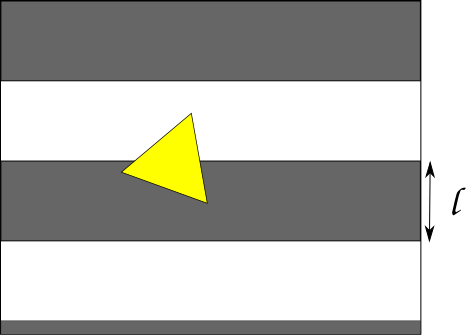
\includegraphics[scale=0.5]{path6509.png}
\caption{\label{couleur} The parallel stripes $2$-colouring}
\end{figure}

For this colouring, the probability of getting the same colour using the first 
process is $\frac13$. This can be shown by direct computation, or we can 
more simply remark that no unit-lengthed equilateral triangle can have its 
three vertices with the same colors. Applying Lemma~\ref{huitre}, we conclude 
that this colouring achieves a probability of $\frac{1}{3}$ indeed.
%CLASSE DE SOLUTIONS?

\subsection{3 colours}
 With three colors, we use the Moser spindle of figure~\ref{color} - a unit 
 distance graph with $m_3(g) = \frac{1}{11}$.
 We similarly get that for $k=3$, $p(c) \geq \frac{1}{11}$ for any valid colouring. 

\begin{figure}[h]
\center
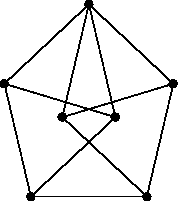
\includegraphics[scale=0.4]{T.png}
\caption{\label{color} The Moser spindle}
\end{figure}

We don't know if the previous bound is optimal. We believe that Figure~\ref{trois} 
can give a rather good $3$-colouring of the plane, for some well chosen length 
of the edge of the hexagons. Rough simulations and optimisation have shown that 
this colouring gives a $\pper(c)$ of about $0.12$ for an edge of length about 
$0.61$, but $0.12$ is still greater than $\frac{1}{11} \simeq 0.091$.
%Still, we did not compute the exact optimum in that case because the 
%estimation is still far away from $\frac{1}{11}$.

\begin{figure}[h]
\center
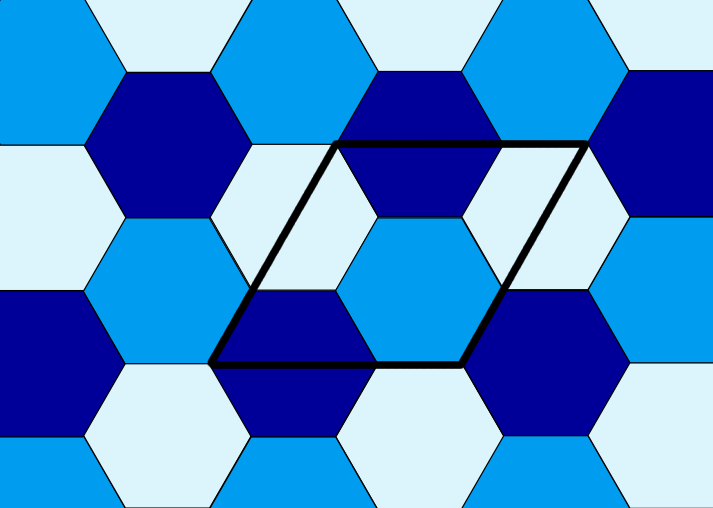
\includegraphics[scale=0.5]{trois.png}
\caption{\label{trois} A hexagonal $3$-colouring and its parallelogram of periodicity}
\end{figure}

\subsection{Connections with the Hadwiger-Nelson problem} \label{hn}
The results shown in this section will be derived using the axiom of choice. 
This is important to notice, since the answer to the Hadwiger-Nelson problem is 
suspected to depend on the set of axioms used. We will use the 
De Bruijn - Erd\H{o}s theorem, established in \cite{erdos}, whose proof uses 
the axiom of choice.
\begin{theo}[De Bruijn - Erdős]
 A graph $G$ can be coloured with $k$ colours iff all of its finite subgraphs 
 can be coloured with $k$ colours.
\end{theo}
In other words, the chromatic number of a graph is the maximum chromatic number 
of its finite subgraphs.

If there exist a unit distance graph (finite by definition) which cannot 
be coloured with $k$ colours, it 
follows from our study that the probability $p(c)$ for $c$ a valid 
$k$-colouring is always greater than a certain constant. Taking the 
contrapositive of this statement and using the De Bruijn-Erdős theorem yields 
corollary~\ref{con}.

\section{Extensions}
\label{ext}
\subsection{Finite table}
\label{fini}

Previously we used periodicity so that we didn't have to worry about the second 
endpoint $B$ falling outside of $\mathbf{P}$, which made things technically easier. We now 
try to require that $B$ fall in $\mathbf{P}$ to match a somewhat more practical 
view: we want to describe the throwing of the needle on an ``actual'' bounded 
table. The first difficulty is to find a natural distribution for our needle.

\begin{process} \label{encore}
Denote by $\mathbf{P}$ an open parallelogram, representing the table. For the 
process to be well defined, we need to assume that $\mathbf{P}$ can contain at
least one needle.
\begin{itemize}
\item Consider the law $\mathcal{L}$ of $(A,B)$ given by Pocess~\ref{premier} on $\P$.
\item Let $(A'',B'')$ be random points in $\P$ following the law
$\mathcal{L}$ conditioned by the event $\{B \in \mathbf{P} \}$.
\end{itemize}
\end{process}

%To evaluate $P(B \in \mathbf{P})$ we need to define the border of a parallelogram~:
\begin{definition}
For $r>0$, let $K(\mathbf{P},r)$ the $r$-wide inner border of $\mathbf{P}$~:
\[K(\mathbf{P},r) = \{ z \in \mathbf{P} \mid d(z,\mathbf{P}^c) < r\} \] 
\end{definition}

\begin{figure}[h]
\center
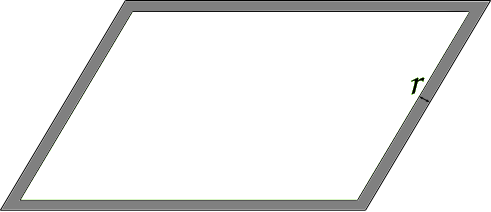
\includegraphics[scale=0.5]{tablefinie.png}
\caption{\label{tablefinie} The set $K(\mathbf{P},r)$ in grey}
\end{figure}

\begin{lemma}\label{choco}
Let $c$ be a $k$-colouring of $\mathbf{P}$. Let $\tilde{c}$ be the periodised version of
$c$ given by repeating $\P$. Let
$\ptable(c) = \Pr(c(A'')=c(B''))$ be the probability given by Process~\ref{encore}. Then 
there is a positive universal constant $\kappa \leq 2$ so that 
$$ | \pper(\tilde{c}) - \ptable(c)| \leq \kappa \frac{\mathcal{A}(K(\mathbf{P},1))}{\mathcal{A}(\mathbf{P})}.$$
\end{lemma}

\begin{proof}
We will show that the inequality is true for $\kappa =2$, but this is probably 
not the best constant.

When $\mathcal{A}(K(\mathbf{P},1)) = \mathcal{A}(\mathbf{P})$ the result is clear,
so we may suppose that these areas differ, which means that there are needles 
inside $\P$ and conditional probabilities will be well defined.

Let $r = \frac{\mathcal{A}(K(\mathbf{P},1))}{\mathcal{A}(\mathbf{P})}$. When 
$r \geq \frac12$ the inequality is obvious, so we will now suppose that 
$r < \frac12$. Consider $(A,B)$ a needle whose law is given by Process~\ref{premier} on $\P$ and let $M$and $N$ be the following events:
$$ M = \{\tilde{c} (A) = \tilde{c} (B) \}, \ N = \{B\notin \P \}.$$
Then $P(N^c) \leq r$, indeed, $B$ can 
be outside of $\mathbf{P}$ only
when $A$ is in $K(\mathbf{P},1)$. Easy computation then shows that
\begin{eqnarray*}
\pper(\tilde{c}) - \ptable(c) & = & P(M) - P(M \mid N) \\
& = & \frac{P(N^c)}{P(N)} \left( P(M\mid N^c) - P(M)\right),
\end{eqnarray*}
and using the fact that $P(N^c) \leq r$ and 
$P(N) \geq 1-r \geq \frac12$ we get 
$$ |\pper(\tilde{c}) - \ptable(c)| \leq 2r.$$
\end{proof}

Since we already have bounds on $\pper$, we can therefore deduce bounds on $\ptable$.
For instance, with $2$ colours, we see that 
$\ptable(c) \geq \frac13 - \kappa \frac{\mathcal{A}(K(\mathbf{P},1))}{\mathcal{A}(\mathbf{P})}$. 
This bound becames sharper as the table parallelogram $\mathbf{P}$ becomes bigger.
\begin{proof}[Proof of Theorem~\ref{ineg2}]
If $c$ is an asymptotic colouring, let $\tilde{c_R}$ be the periodised version of $c_{|[-R;R]^2}$ (that is, restrict $c$ to $[-R;R]^2$ and tile the plane by repeating this square). By lemma~\ref{choco},
\begin{equation} \label{estim}
|\pper(\tilde{c_R}) - \ptable(c_{|[-R;R]^2}) | \leq \kappa \frac{\mathcal{A}(K([-R;R]^2,1))}{\mathcal{A}([-R;R]^2)} \leq \kappa \frac{4R}{R^2} = \frac{4\kappa}{R}.
\end{equation}
But $\ptable(c_{|[-R;R]^2}) = \frac{\lambda (\M_{[-R;R]^2})}{\lambda (\N_{[-R;R]^2})}$ (see definition~\ref{defas} for notations) and this ratio converges to $p(c)$ as $R\rightarrow +\infty$. The bounds on $\pper(\tilde{c_R})$ given by theorem~\ref{ineg} and the estimate~(\ref{estim}) yield theorem~\ref{ineg2}.
\end{proof}

It may seem a bit odd to chose a square to define asymptotic colourings in definition~\ref{defas}. One could have, for instance, replaced $[-R,R]^2$ by the disk $D(O,R)$ in this definition. The advantage of the square is that it made the previous proof easier, given that periodic colourings were already studied. Getting similar results for a disk (or with any open set bounded by a smooth curve) would require a result similar to lemma~\ref{huitre} with an estimation similar to the one in lemma~\ref{choco}.

Still, it should be noted that the value of $p(c)$ defined by asymptotics on different shapes may differ. For instance, consider the 2-colouring of figure \ref{contrex} where stripes are $\frac{\sqrt{3}}{2}$ appart. In the striped region the probability is approximately $\frac13$ (see section \ref{2col}), and it is $1$ in the rest of the plane. So $p(c)$ is related to the fraction of a square (resp. disk) occupied by the striped region, and this fraction is different in these two cases.

\begin{figure}[h]
\center
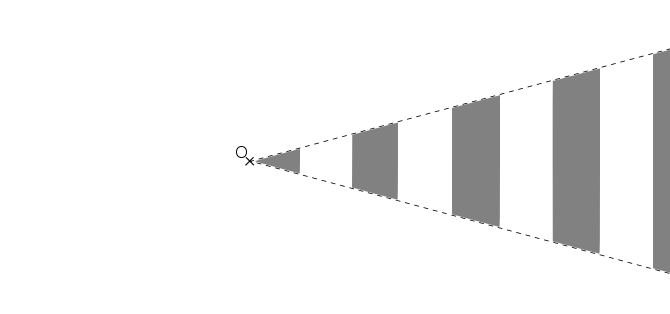
\includegraphics[scale=0.5]{contrex.png}
\caption{\label{contrex} An asymptotic 2-colouring of the plane}
\end{figure}

However, the unequality of theorem~\ref{ineg2} should remain true for these different possible values of asymptotic $p(c)$'s.

\subsection{Higher dimensions}
\label{dim}
The previous considerations can be extended to dimension $d \geq 3$, however, 
it becomes more complicated to write down. We have to consider a basis of 
vector leaving our colouring unchanged ; we still denote by $\mathbf{P}$ the 
parallelepiped induced by these vectors.

The first process for choosing a needle now consist in~: 
\begin{itemize}
	\item choosing one point uniformly in the parallelepiped $ \mathbf{P} $ as 
	one point of the needle~;
	\item choosing independently one point uniformly on the unit sphere 
	$S^{d-1}$, to give the relative position of the second point.
\end{itemize}

Sending a unit-length graph on the $d$-dimensional space becomes a bit more 
tricky. We have to choose one initial point in $ \mathbf{P} $, and an independent 
rotation of the graph ; this can be achieved 
by using the Haar measure of $SO(d)$ uniformly. The second process now consists 
in: rotating the graph thanks to the matrix of $SO(d)$ chosen, translating it 
to the point of $\mathbf{P}$ chosen, and chosing one of the 
edges independently as your needle.

One can verify that the proof of Lemma~\ref{huitre} adapts to that definitions. 
%It means that previous results still hold - namely, the probability that both 
%ends fall on the same colour remains the same for the two processes.
Crucial 
points of the proof are the invariance of the Haar measure under matrix product, and the 
fact that the image measure of said Haar measure by the application 
$M\mapsto Mv$, where $v$ is a given unit vector, is the uniform Lebesgue 
measure of $S^{d-1}$.

Thus, to find lower bonds on our probability, the same techniques may be applied 
in any finite dimension. For instance, in dimension $d$ with $2$ colours,
the probability to get a monochromatic  
needle is always at least $\frac{1}{3}$ because of the equilateral triangle. 
We still don't know whether the bound of $\frac{1}{3}$ is achieved or not in 
dimension $3$ or more.

Remark that in higher dimension, better minorations may be provided by 
Theorems~\ref{ineg}~and~\ref{ineg2}, since new graphs can 
become unit-length. For example, with $3$ colours in dimension $3$, the regular 
tetrahedron gives a better lower bound 
of $\frac 1 6 >\frac 1 {11}$. More generally, considering the complete graph 
$K_{k+1}$ in dimension $k$ (also known as the regular $k+1$-simplex). It is a unit distance graph and is not $k$-colourable, so the 
probability of getting a monochromatic needle is at least $\frac{1}{\binom{k+1}{2}}$ 
for $k$ colours in dimension $k$.

\subsection*{Acknowledgements}
We are very grateful to David Naccache for his constant help in the writing of
this paper, and to Eric Brier for many ideas and insight on the subject of 
unit distance graphs.

\bibliographystyle{abbrv}
\bibliography{Tiling}

\end{document}
